\setmainfont{Noteworthy}
%TODO: provide your details here.
\begin{frame}
    \frametitle{About Your Fellows}
    \begin{itemize}
        \item Hi there! We are \textcolor{blue}{\textbf{ Mihab Khan}  \textcolor{black}{and}\textbf{ Maira Fatima}}.
        \item We are Associate Students at ITU.
    \end{itemize}
\end{frame}
\begin{frame}{Graph of Nodes C, D, E, F, T}

\textbf{Note:} We can write the table in any order, but maintaining the same order makes interpretation easier.
    \begin{center}
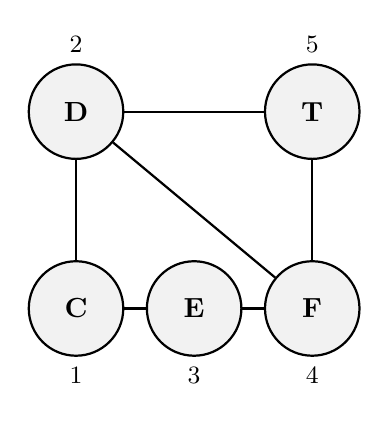
\begin{tikzpicture}[node distance=2.5cm, thick]
    % Node style
    \tikzstyle{vertex}=[circle, draw=black, fill=gray!10, minimum size=1.2cm, font=\bfseries]

    % Nodes with labels
    \node[vertex, label=below:{\small 1}] (C) at (0,0) {C};
    \node[vertex, label=above:{\small 2}] (D) at (0,2.5) {D};
    \node[vertex, label=above:{\small 5}] (T) at (3,2.5) {T};
    \node[vertex, label=below:{\small 4}] (F) at (3,0) {F};
    \node[vertex, label=below:{\small 3}] (E) at (1.5,0) {E};

    % Undirected Edges
    \draw (C) -- (D);
    \draw (D) -- (T);
    \draw (T) -- (F);
    \draw (C) -- (E);
    \draw (E) -- (F);
    \draw (D) -- (F);
\end{tikzpicture}
\end{center}
\end{frame}
\begin{frame}{Shortest Path}
\textbf{Find the distance from node $i$ to $j$, but there will be  restricted subset of vertices that can be visited while finding the shortest path.}

\vspace{1em}

\textbf{When all vertices are allowed in the graph, the shortest path is found.}
\vspace{1em}

\begin{center}
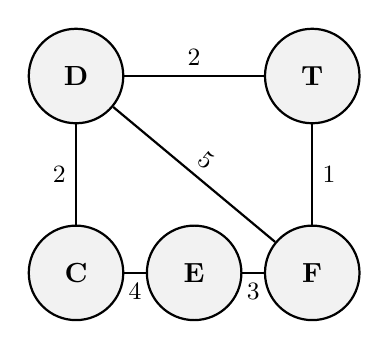
\begin{tikzpicture}[node distance=2.5cm, thick]
    % Node style
    \tikzstyle{vertex}=[circle, draw=black, fill=gray!10, minimum size=1.2cm, font=\bfseries]

    % Nodes
    \node[vertex] (C) at (0,0) {C};
    \node[vertex] (D) at (0,2.5) {D};
    \node[vertex] (T) at (3,2.5) {T};
    \node[vertex] (F) at (3,0) {F};
    \node[vertex] (E) at (1.5,0) {E};

    % Undirected Edges with weights
    \draw (C) -- (D) node[midway, left] {\small 2};
    \draw (D) -- (T) node[midway, above] {\small 2};
    \draw (T) -- (F) node[midway, right] {\small 1};
    \draw (C) -- (E) node[midway, below] {\small 4};
    \draw (E) -- (F) node[midway, below] {\small 3};
    \draw (D) -- (F) node[midway, sloped, above] {\small 5};
\end{tikzpicture}
\end{center}

\vspace{1em}
\textit{This graph could have been negative, and it wouldn't have affected anything (process/solution).}
\end{frame}




\begin{frame}{\textit{d(i, j, 0)}}

\centering

\vspace{1em}

\begin{tabular}{c|ccccc}
     & C & D & E & F & T \\
    \hline
    C & 0  \\
    D & 2  \\
    E & 4  \\
    F & $\infty$  \\
    T & $\infty$  \\
\end{tabular}\\
\vspace{1em}
\vspace{1em}
\textit{Diagonal is on zero, so you don't have to go anywhere to visit the vertex where it is standing on (i.e. distance from D to D is 0 , C to C is 0 , E to E is 0 etc.)}
\vspace{1em}

\end{frame}

\begin{frame}{\textit{d(i, j, 0)}}

\centering

\vspace{1em}

\begin{tabular}{c|ccccc}
     & C & D & E & F & T \\
    \hline
    C & 0 & 2\\
    D & 2 & 0\\
   E & 4 & $\infty$ \\
   F & $\infty$ & 5 \\
    T & $\infty$ & 2  \\
\end{tabular}

\vspace{1em}

\end{frame}

\begin{frame}{\textit{d(i, j, 0)}}

\centering

\vspace{1em}

\begin{tabular}{c|ccccc}
     & C & D & E & F & T \\
    \hline
    C & 0 & 2 & 4 \\
    D & 2 & 0 & $\infty$\\
   E & 4 & $\infty$ & 0  \\
   F & $\infty$ & 5 & 3\\
    T & $\infty$ & 2 & $\infty$\\
\end{tabular}

\vspace{1em}

\end{frame}

\begin{frame}{\textit{d(i, j, 0)}}

\centering

\vspace{1em}

\begin{tabular}{c|ccccc}
     & C & D & E & F & T \\
    \hline
     C & 0 & 2 & 4 & $\infty$ \\
   D & 2 & 0 & $\infty$ & 5 \\
    E & 4 & $\infty$ & 0 & 3 \\
   F & $\infty$ & 5 & 3 & 0 \\
   T & $\infty$ & 2 & $\infty$ & 1\\
\end{tabular}

\vspace{1em}

\end{frame}

\begin{frame}{\textit{d(i, j, 0)}}

\centering

\vspace{1em}

\begin{tabular}{c|ccccc}
     & C & D & E & F & T \\
    \hline
    C & 0 & 2 & 4 & $\infty$ & $\infty$ \\
    D & 2 & 0 & $\infty$ & 5 & 2 \\
    E & 4 & $\infty$ & 0 & 3 & $\infty$ \\
    F & $\infty$ & 5 & 3 & 0 & 1 \\
    T & $\infty$ & 2 & $\infty$ & 1 & 0 \\
\end{tabular}

\vspace{1em}
\vspace{1em}

\vspace{1em}
\end{frame}

\begin{frame}{\textit{d(i, j, 1)} }

\vspace{0.5em}
\textbf{$d(i, j, 1)$: Allowed to visit vertex 1 {\textcolor{myNewColorA}{\{C\}}}}

\vspace{1.5em}

\begin{tikzpicture}[remember picture, overlay]
    \node[anchor=north west] (table) at (0,0) {
        \begin{tabular}{c|ccccc}
             & C & D & E & F & T \\
            \hline
            C & 0 & 2 & 4 & $\infty$ & $\infty$ \\
            D & 2 & 0 & \tikz[baseline]{\node[anchor=base,inner sep=0pt](DE){\textcolor{red}{6}};} & 
                  \tikz[baseline]{\node[anchor=base,inner sep=0pt](DF){\textcolor{blue}{5}};} & 2 \\
            E & 4 & 6 & 0 & 3 & $\infty$ \\
            F & $\infty$ & 5 & 3 & 0 & 1 \\
            T & $\infty$ & 2 & $\infty$ & 1 & 0 \\
        \end{tabular}
    };

    % Arrow and annotation for D,E
    \draw[->, thick, red] (DE) -- ++(4.3,0)
        node[right, text width=5cm, align=left] {
            $d(D,E,\{C\})$\\
            $= d(D,C,\{\}) = 2$\\
            $+ d(C,E,\{\}) = 4$\\
            $= 6$
        };

    % Arrow and annotation for D,F
    \draw[->, thick, blue] (DF) -- ++(4.3,-1.6)
        node[right, text width=5.5cm, align=left] {
            $d(D,F,1) = \min(5,$\\
            $\quad d(D,C,0)=2 +$\\
            $\quad d(C,F,0)=\infty)$\\
            $= \min(5,\ \infty)$\\
            $= 5$
        };

\end{tikzpicture}

\vspace{10em} % Adjust spacing to move below TikZ

\text{
\begin{array}{l}
\bullet\quad \text{C} \rightarrow \text{C} = 0 \quad \text{(same node)} \\
\bullet\quad \text{D} \rightarrow \text{C} = 2 \\
\bullet\quad \text{E} \rightarrow \text{C}= 4 \\
\bullet\quad \text{F and T have no direct path to C, so it's } \infty \\
\text{ Only direct paths or paths going through C are considered.}
\end{array}
}

\end{frame}

\begin{frame}{\textit{d(i, j, 2)}}

\centering

\vspace{1em}

\textbf{$d(i, j, 1)$: Allowed to visit 2 vertices {\textcolor{myNewColorA}{\{C,D\}}}}

\begin{tabular}{c|ccccc}
     & C & D & E & F & T \\
    \hline
  C & 0 & 2 & 4 & 7 & 4 \\
  D & 2 & 0 & 6 & 5 & 2 \\
  E & 4 & 6 & 0 & 3 & 8 \\
  F & 7 & 5 & 3 & 0 & 1 \\
  T & 4 & 2 & 8 & 1 & 0 \\
\end{tabular}

\vspace{1em}

\textcolor{gray}{\text{Assadullah volunteered to solve the matrix}}



\end{frame}

\begin{frame}{\textit{d(i, j, 3)}}

\centering

\vspace{1em}

\textbf{$d(i, j, 3)$: Allowed to visit 3 vertices {\textcolor{myNewColorA}{\{C,D,E\}}}}

\begin{tabular}{c|ccccc}
     & C & D & E & F & T \\
    \hline
    C & 0 & 2 & 4 & 7 & 4 \\
    D & 2 & 0 & 6 & 5 & 2 \\
    E & 4 & 6 & 0 & 3 & 8 \\
    F & 7 & 5 & 3 & 0 & 1 \\
    T & 4 & 2 & 8 & 1 & 0 \\
\end{tabular}

\vspace{1em}

\textcolor{gray}{\text{Saifullah volunteered to solve the matrix}}\\
\vspace{1em}
\textit{Asharib proposed the question:} \\
\textquotedblleft If there are no $\infty$ values, does that mean we have found all shortest paths?\textquotedblright \\[1em]

\textit{Professor replied:} \\
\textquotedblleft Just because there is no $\infty$, it doesn't mean that every path is the shortest.\textquotedblright \\[1em]

\textbf{Hence, we need to perform all steps till the end.}
\end{frame}



\begin{frame}{\textit{d(i, j, 4)}}

\centering
\textit{To make it interesting , professor erased the graph from board.}
\vspace{1em}

\textbf{$d(i, j, 4)$: Allowed to visit 4 vertices {\textcolor{myNewColorA}{\{C,D,E,F\}}}}

\begin{tabular}{c|ccccc}
     & C & D & E & F & T \\
    \hline
    C & 0 & 2 & 4 & 7 & 4 \\
    D & 2 & 0 & 6 & 5 & 2 \\
    E & 4 & 6 & 0 & 3 & \textcolor{red} 4 \\
    F & 7 & 5 & 3 & 0 &1 \\
    T & 4 & 2 & \textcolor{red}4 & 1 & 0 \\
\end{tabular}

\vspace{1em}

\textcolor{gray}{\text{Wasif volunteered to solve the matrix}} \\
\vspace{1em}
\begin{minipage}{\linewidth}

\textit{He mentioned that rest of the matrix will remain same just the distance b/w E \& T will be updated.}
\end{minipage}



\end{frame}

\begin{frame}{\textit{d(i, j, 5)}}

\centering

\vspace{1em}

\textbf{$d(i, j, 5)$: Allowed to all vertices 
{\textcolor{myNewColorA}{\{C,D,E,F,T\}}}}
\begin{tabular}{c|ccccc}
     & C & D & E & F & T \\
    \hline
    C & 0 & 2 & 4 & 7 & 4 \\
    D & 2 & 0 & 6 & 5 & 2 \\
    E & 4 & 6 & 0 & 3 & 4 \\
    F & 7 & 5 & 3 & 0 & 1 \\
    T & 4 & 2 & 4 & 1 & 0 \\
\end{tabular}

\vspace{1em}

\textit{Matrix will not change because all shortest paths are discovered}

\end{frame}

\begin{frame}{Floyd-Warshall}
\textbf{Algorithm:}
\[
d_{ij} =
\begin{cases}
w_{ij} & \text{if } w_{ij} \neq 0\quad \text{\textit{\textcolor{gray}{(if there is a edge, edge weight is the shortest path)}}} \\
\infty & \text{otherwise}\quad \text{\textit{\textcolor{gray}{(if no edge, weight is }$\infty$\textcolor{gray}{)}}}
\end{cases}
\]
\begin{align*}
\text{for } k &= 1 \text{ to } n:\\
\quad \text{for } i &= 1 \text{ to } n; \\
\quad\quad \text{for } j &= 1 \text{ to } n; \\
\quad\quad\quad d(i,j) &= \min(d(i,j),\ d(i,k) + d(k,j))\\
\quad\quad\quad\quad\quad \text{ ret d } 
\end{align*}
\text{\textit{\textcolor{gray}{(This algo is giving the distance between vertices not the shortest path.)}}} \\
\vspace{1em}
\textbf{H.W Q:How do we use Floyd-Warshall to find negative cycles in graph?}\\
\textbf{H.W Q:Rewrite this algo to find shortest path?}
\end{frame}

\begin{frame}{Dynamic Programming}
Dynamic Programming is used to solve optimization problems.

\vspace{0.5em}
\textit{- Design paradigm} \\
\textit{- Used in special circumstances}

\vspace{1em}
\textit{\textcolor{gray}{
Back in the 1950s, a person introduced a method with a technical and complex name. 
To make it sound more appealing, especially for funding purposes in the US, he renamed it "Dynamic Programming". 
The new name helped it gain popularity. Interestingly, the name has nothing to do with the actual method.There is neither anything "dynamic" nor any "programming" involved in the technique, yet the term "DP" stuck, and that is what everyone started calling it.
}}
\end{frame}

\begin{frame}{Dynamic Programming}
\textbf{Requirement:}\\
\text{1) The problem should have recursive aspect.}\\ \textit{\textcolor{gray}{(You should be able to write problem as recurrence)}}\\
\text{2)Over-Lapping Subproblem}
\end{frame}

\begin{frame}{Fibonacci Recursive}
\textit{\textcolor{gray}{(Without Dynamic Programming, you'd typically write a recursive function, which can be inefficient. Instead, using DP is a better approach.)}}\\
\vspace{1em}
    \textbf{Recursive Function Example:}

    \vspace{1em}
    \texttt{fib(n)} \\
    \texttt{\{} \\
    \hspace{1em} \texttt{if (n <= 2)} \\
    \hspace{2em} \texttt{return n - 1;} \\
    \hspace{1em} \texttt{else} \\
    \hspace{2em} \texttt{return fib(n - 1) + fib(n - 2);} \\
    \texttt{\}}

    \end{frame}
\begin{frame}
\itshape \textcolor{gray}{(This algorithm computes the distance between vertices, not the shortest path.)} \\
\vspace{1em}
\textbf{Recursive Tree for \texttt{f(n)}:}
\[
\hspace*{-2em} % shift entire tree left
\begin{array}{c}
f(n) \\
\quad / \qquad \quad \backslash \quad \\
f(n-1) \qquad \quad f(n-2) \\
\quad \quad / \quad \quad \backslash \qquad \qquad \quad / \quad \quad \backslash \quad \\
\qquad f(n-2) \qquad f(n-3) \quad f(n-3) \quad f(n-4) \\
/ \quad \quad \backslash \quad \quad \quad \quad \quad \quad  \quad / \quad \quad \backslash \\
f(n-3) \quad \quad f(n-4) \quad \quad f(n-4) \quad f(n-5)
\end{array}
\]
\textbf{Overlapping Subproblems} \\
Dynamic programming exploits this overlap. Instead of re-computing the same subproblems, we solve each one once, store the result, and reuse it when needed.
\end{frame}

\begin{frame}{Memoization}
\textbf{memo - means small letter}\\
 \vspace{1em}
\textit{DP says that write this thing on memo and use that memo whenever you need.}\\
 \vspace{1em}
    \texttt{fib(n)} \\
    \texttt{\{} \\
    \hspace{1em} \texttt{memo = []} \\
    \hspace{2em} \texttt{memo[0] = 0} \\
    \hspace{2em} \texttt{memo[1] = 1} \\
    \hspace{1em} \texttt{for(i = 2; i < n; i++) \{} \\
    \hspace{2em} \texttt{memo[i] = memo[i-1] + memo[i-2]} \\
    \hspace{1em} \texttt{\}} \\
    \hspace{1em} \texttt{return memo[n-1]} \\
    \texttt{\}}\\
\textbf{Time Complexity is O(n).}\\
\text{Difference in recursive and dynamic programming is time complexity}
\end{frame}
\begin{frame}
\small
\textit{\textcolor{gray}{Hamza pointed out it increases space complexity}} \\
\vspace{1em}
\textbf{Professor replied:} \\
Dynamic programming has a memory impact, storing all solutions. 
In this case, we maintain a stack of at least size $n$. 
We make $n$ calls for $f(n)$, we store $f(n-2)$, $f(n-3)$, etc., so the entire stack is linear. 
However, with a clever approach, you can achieve the same result using a constant amount of memory. 
In general, dynamic programming requires a table that typically requires a linear amount of memory.
\end{frame}
\begin{frame}{Real-World Context: DNA and Disease Cure Discovery}
\begin{itemize}
    \item In the fight against emerging diseases, researchers often need rapid cures for newly discovered pathogens.
    \item These pathogens have DNA/RNA sequences that can be compared with those of known viruses or bacteria.
\end{itemize}

\vspace{0.4cm}

\textbf{Why Compare DNA Sequences?}
\begin{itemize}
    \item DNA carries biological instructions.
    \item Similar DNA → similar biological behavior and possible treatment response.
\end{itemize}
\end{frame}

\begin{frame}{Edit Distance and Drug Development}
\textbf{Edit Distance as a Measure of Similarity}
\begin{itemize}
    \item Counts insertions, deletions, substitutions needed to convert one DNA sequence into another.
    \item Small edit distance $\Rightarrow$ high similarity $\Rightarrow$ possibly similar treatment.
\end{itemize}

\vspace{0.3cm}

\textbf{Using Known Treatments:}
\begin{itemize}
    \item Genetically close pathogens (low edit distance) suggest reuse or slight modification of existing drugs.
\end{itemize}

\vspace{0.3cm}

\textbf{Optimizing Drug Design:}
\begin{itemize}
    \item Bioinformatics tools use edit distance to align sequences and highlight mutations.
    \item Predict impact of mutations and suggest changes to drugs.
\end{itemize}
\end{frame}


\begin{frame}{Why Efficient Algorithms Matter}
\begin{itemize}
    \item DNA sequences can be millions of base pairs long.
    \item Brute-force comparison is too slow.
    \item Dynamic programming-based edit distance algorithms make large-scale comparisons feasible.
\end{itemize}

\vspace{0.4cm}

\textit{“Imagine you’re a computational biologist working on a virus like COVID-25. You're given its genome. Your task: Find which known virus it is genetically closest to. How do you measure that?”} \\
\vspace{0.2cm}
\hfill $\Rightarrow$ Leads directly into the Edit Distance Problem
\end{frame}
\begin{frame}{Example}


    \small
    \textbf{Example:}\\
    \text{String 1: AAAACTGG}\\
    \text{String 2: GCATG}\\
    \textit{We are allowed to:}\\
    \begin{itemize}
        \item insert letter (cost = 1)
        \item delete letter (cost = 1)
        \item Exchange/Swap letter (cost = 1)
        \item Match (cost = 0)
    \end{itemize}
    \text{This problem becomes very easy with dynamic programming}\\
    \vspace{0.5cm}
  \textcolor{gray}{\text{It is not a string matching problem}\\
   \text{because none of the strings are ever gonna be exactly same}}


\end{frame}

\begin{frame}{Example: Solution Steps}
    \small
    \begin{enumerate}
        \item \textbf{Match: "A" (String 1) with "A" (String 2)}\\
              \textit{No change needed.}
        \item \textbf{Delete: "A" (String 1)}\\
              \textit{String 1 becomes "AACTGG".}
        \item \textbf{Delete: "A" (String 1)}\\
              \textit{String 1 becomes "ACTGG".}
        \item \textbf{Match: "C" (String 1) with "C" (String 2)}\\
              \textit{No change needed.}
        \item \textbf{Exchange: Swap "T" and "G" (String 1)}\\
              \textit{String 1 becomes "ACGTTG".}
        \item \textbf{Match: "G" (String 1) with "G" (String 2)}\\
              \textit{No change needed.}
        \item \textbf{Delete: "T" (String 1)}\\
              \textit{String 1 becomes "ACGTG".}
        \item \textbf{Delete: "G" (String 1)}\\
              \textit{String 1 becomes "ACGT".}
        \item \textbf{Insert: "T" (String 2)}\\
              \textit{String 1 becomes "GCATG".}
    \end{enumerate}
\end{frame}
\begin{frame}{Example: Final Result}
    \small
    \textbf{Final Result:}\\
    \begin{itemize}
        \item \textbf{Operations}:
        \begin{itemize}
            \item 3 Matches
            \item 4 Deletions
            \item 1 Insertion
            \item 1 Exchange
        \end{itemize}
        \item \textbf{Total Operations: 9}
        \item \textbf{Total Cost}: \( 0 \times 3 + 1 \times 4 + 1 \times 1 + 1 \times 1 = 6 \)
        \item \textbf{Distance}: 
              \[
              d(\text{String 1}, \text{String 2}) = 4 \, (\text{deletions}) + 1 \, (\text{insertion}) + 1 \, (\text{exchange}) = 6
              \]
              So, the distance \( d(\text{String 1}, \text{String 2}) = 6 \).
    \end{itemize}
\end{frame}